\section{Targeted follow-up studies}

The next layer of the project is no longer a generic graph-family comparison. It is a set of targeted tests motivated by the first-pass atlas: a refined disorder scan for the chain, a denser size scan for the ring, a controlled ring study that separates parity from distance to the trap, and a sink-position sweep for all currently implemented topologies.

\begin{figure}[t]
\centering
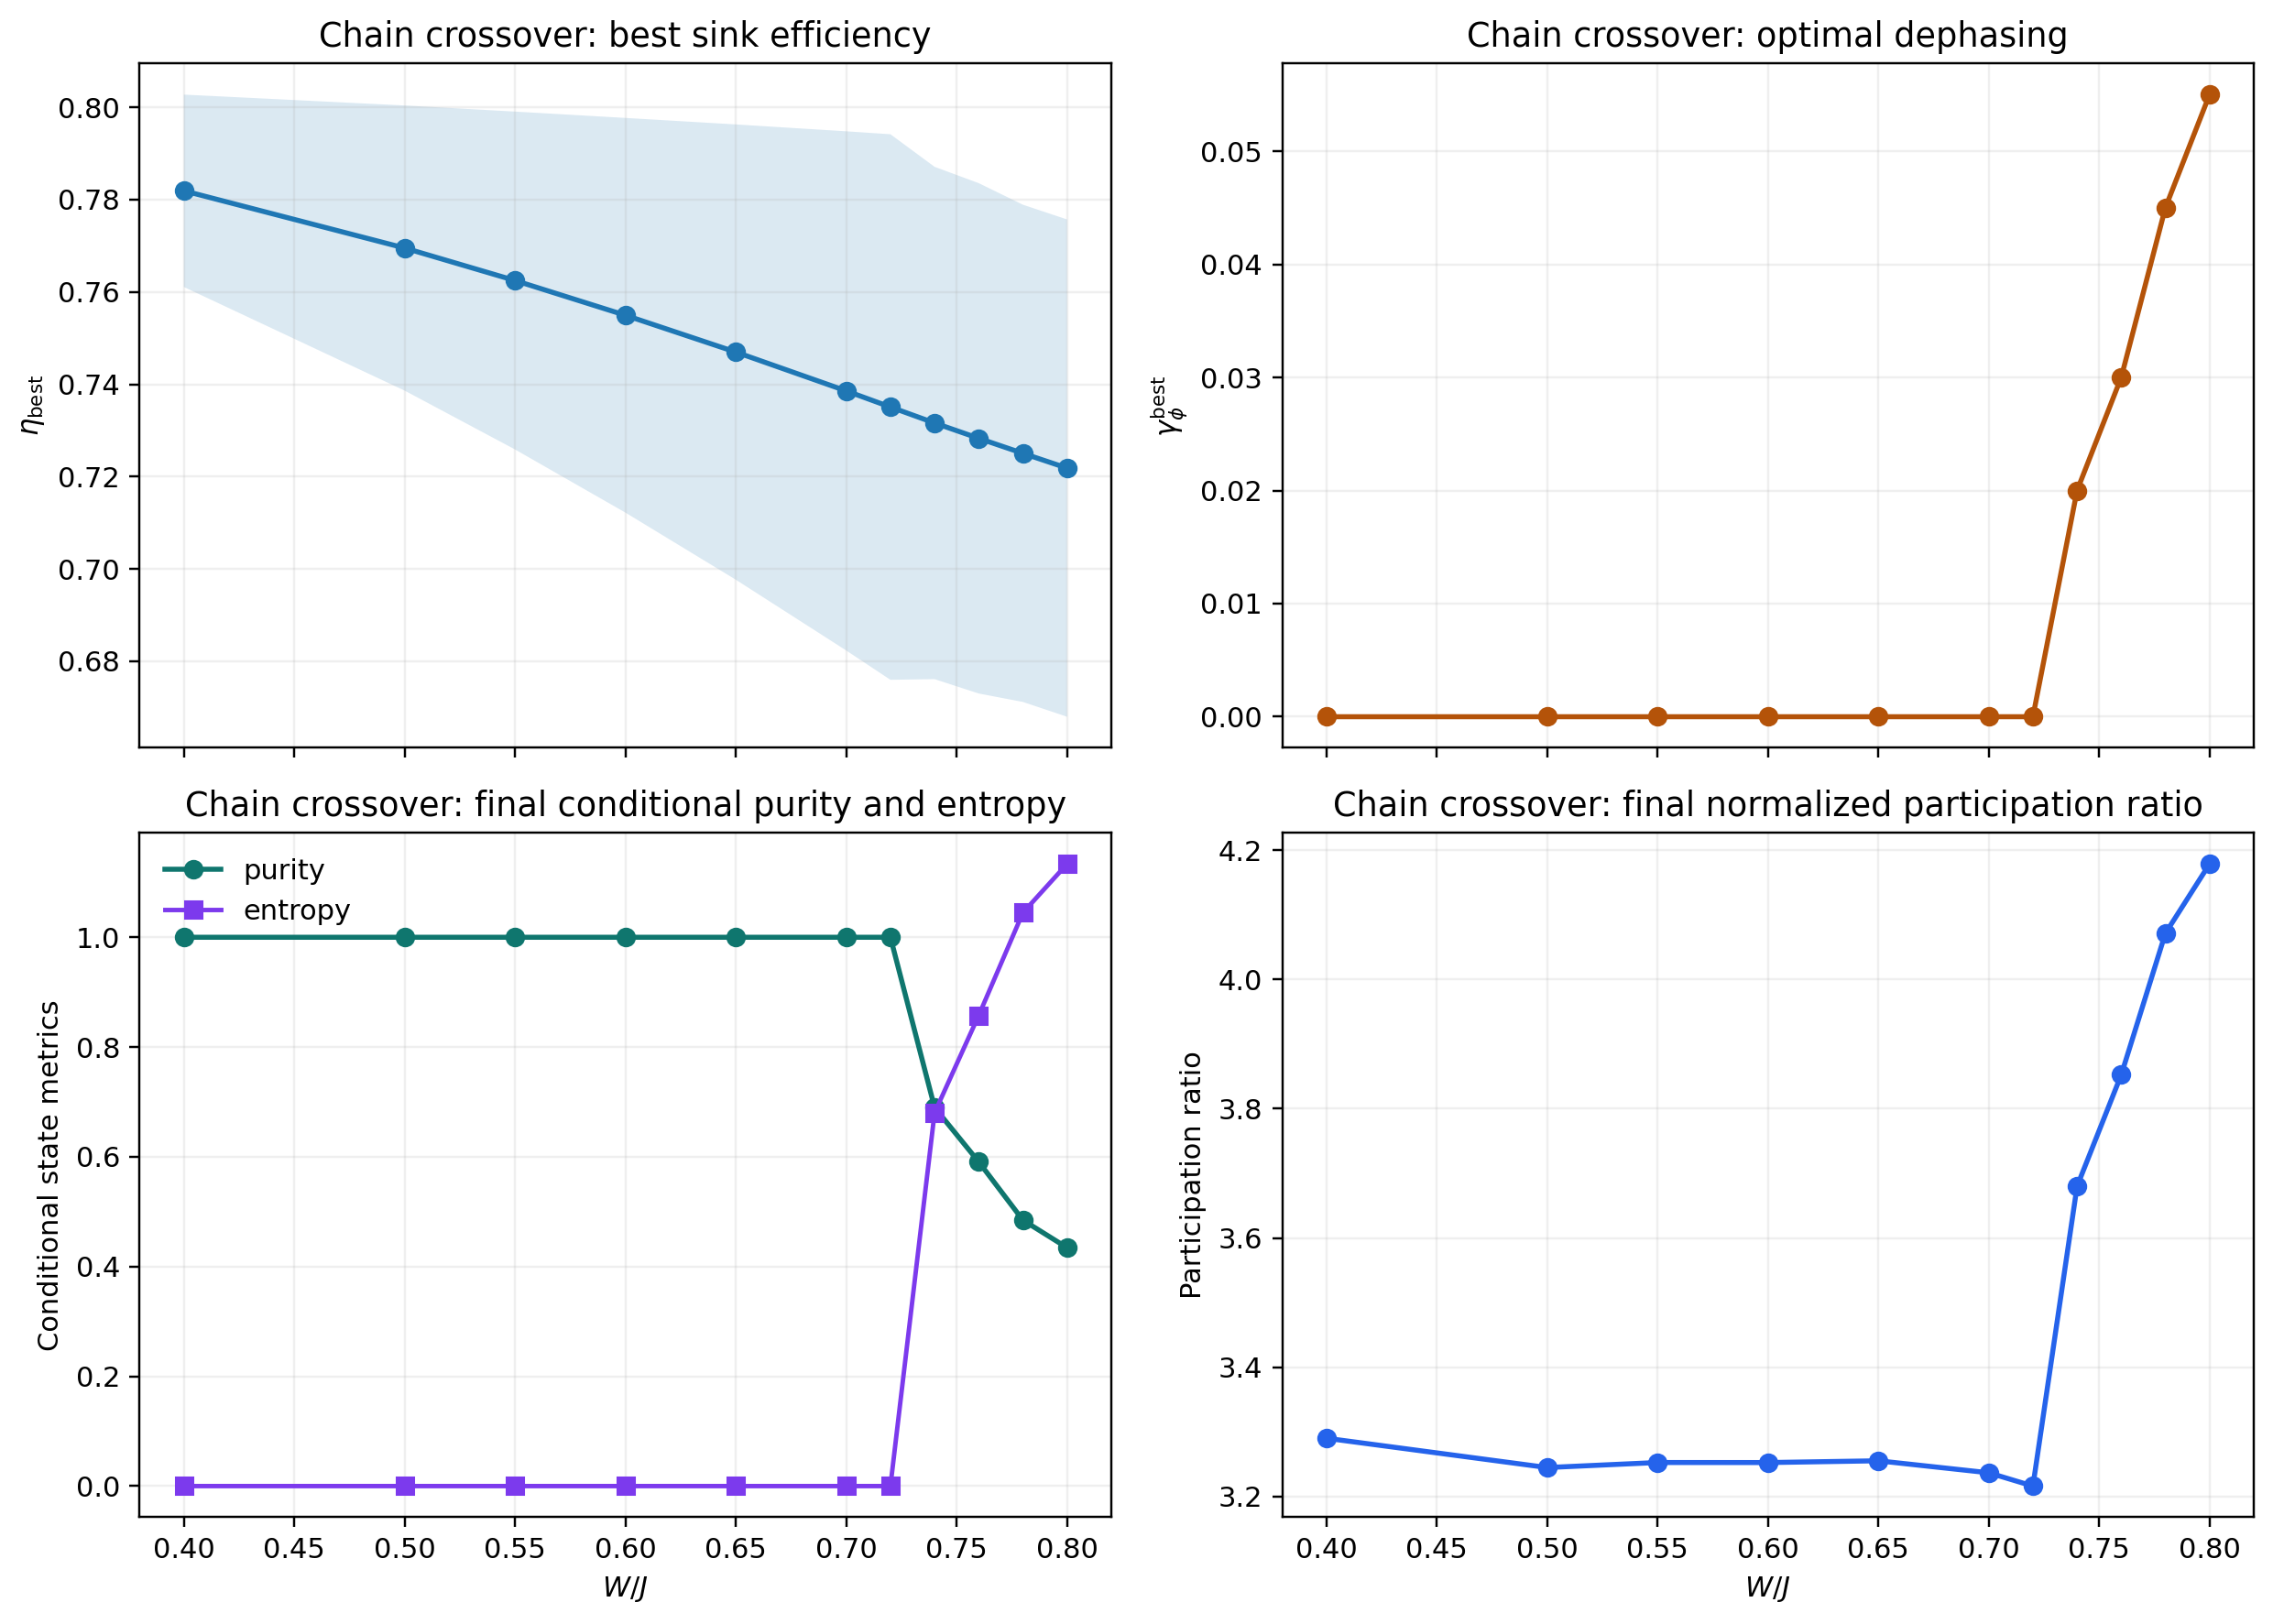
\includegraphics[width=0.86\textwidth]{../../outputs/transport_networks/targeted_studies/latest/figures/chain_crossover_refined.png}
\caption{Refined chain crossover study. Top-left: best sink efficiency versus $W/J$. Top-right: optimal dephasing versus $W/J$. Bottom panels: final conditional purity, entropy, and participation ratio at the transport optimum.}
\end{figure}

\begin{figure}[t]
\centering
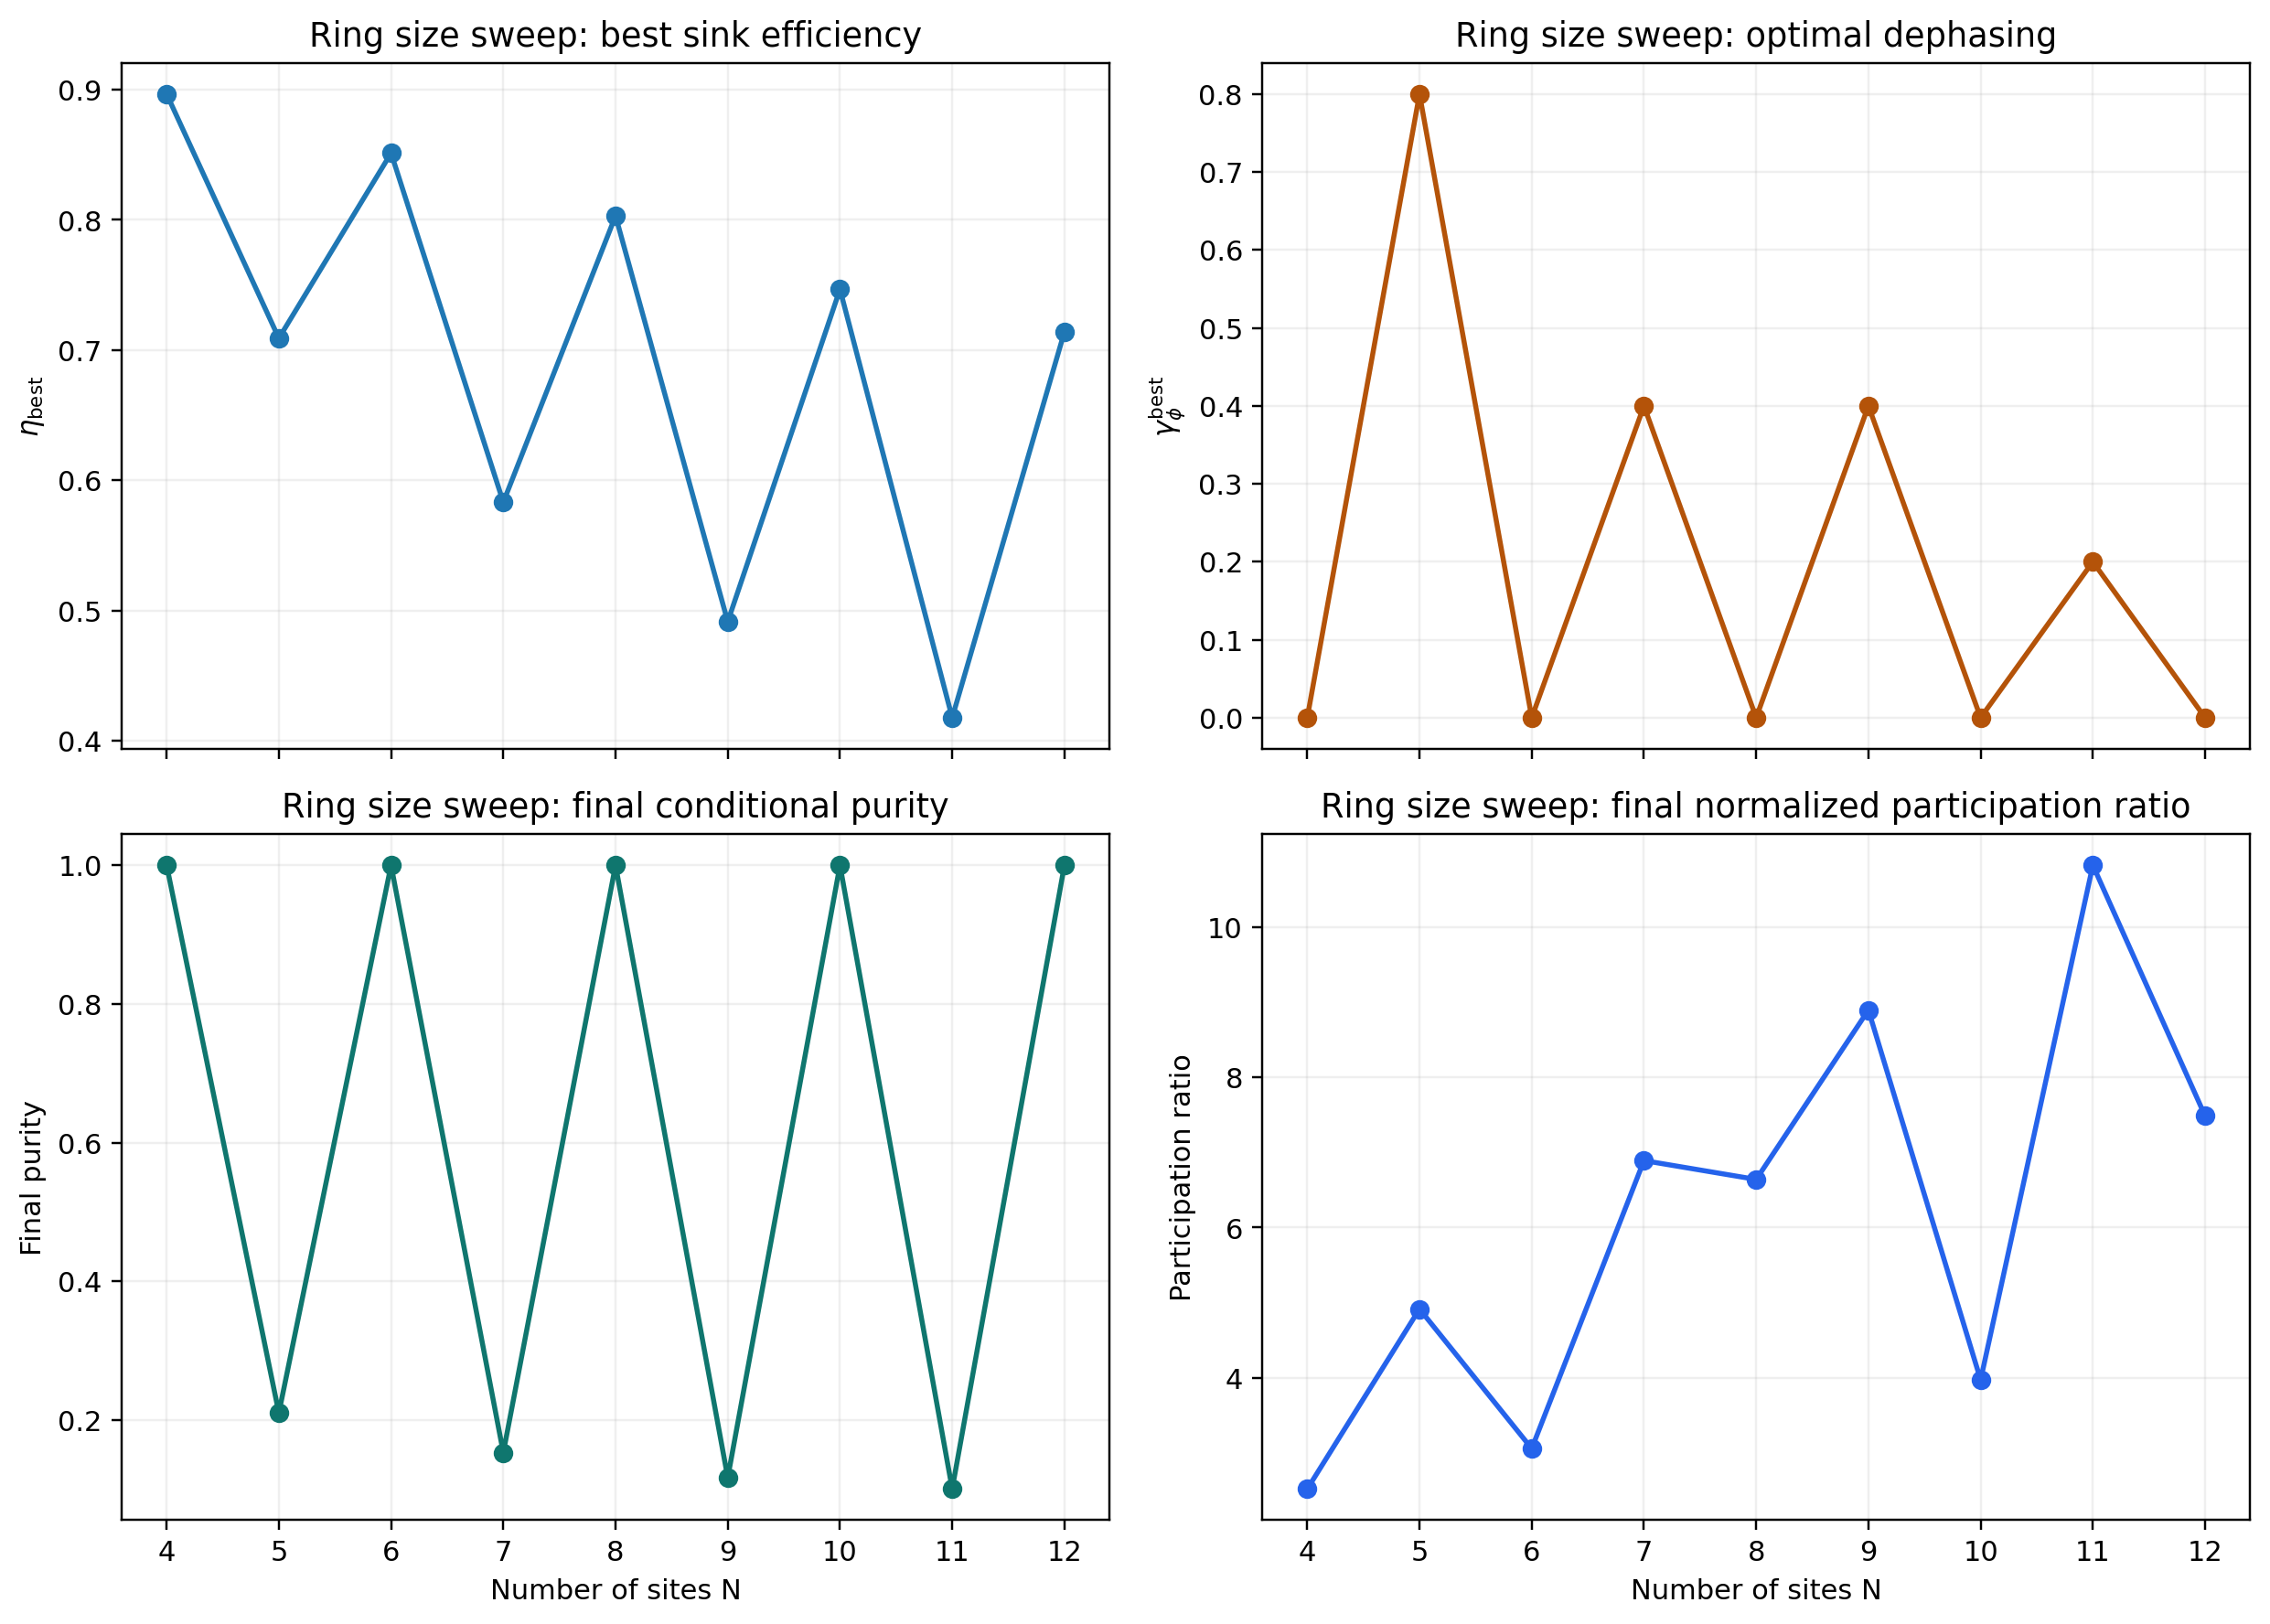
\includegraphics[width=0.86\textwidth]{../../outputs/transport_networks/targeted_studies/latest/figures/ring_size_refined.png}
\caption{Refined ring-size study. The goal is to test whether the original alternation between coherent-optimal and intermediate-optimal behavior is a real parity/symmetry effect.}
\end{figure}

\begin{figure}[t]
\centering
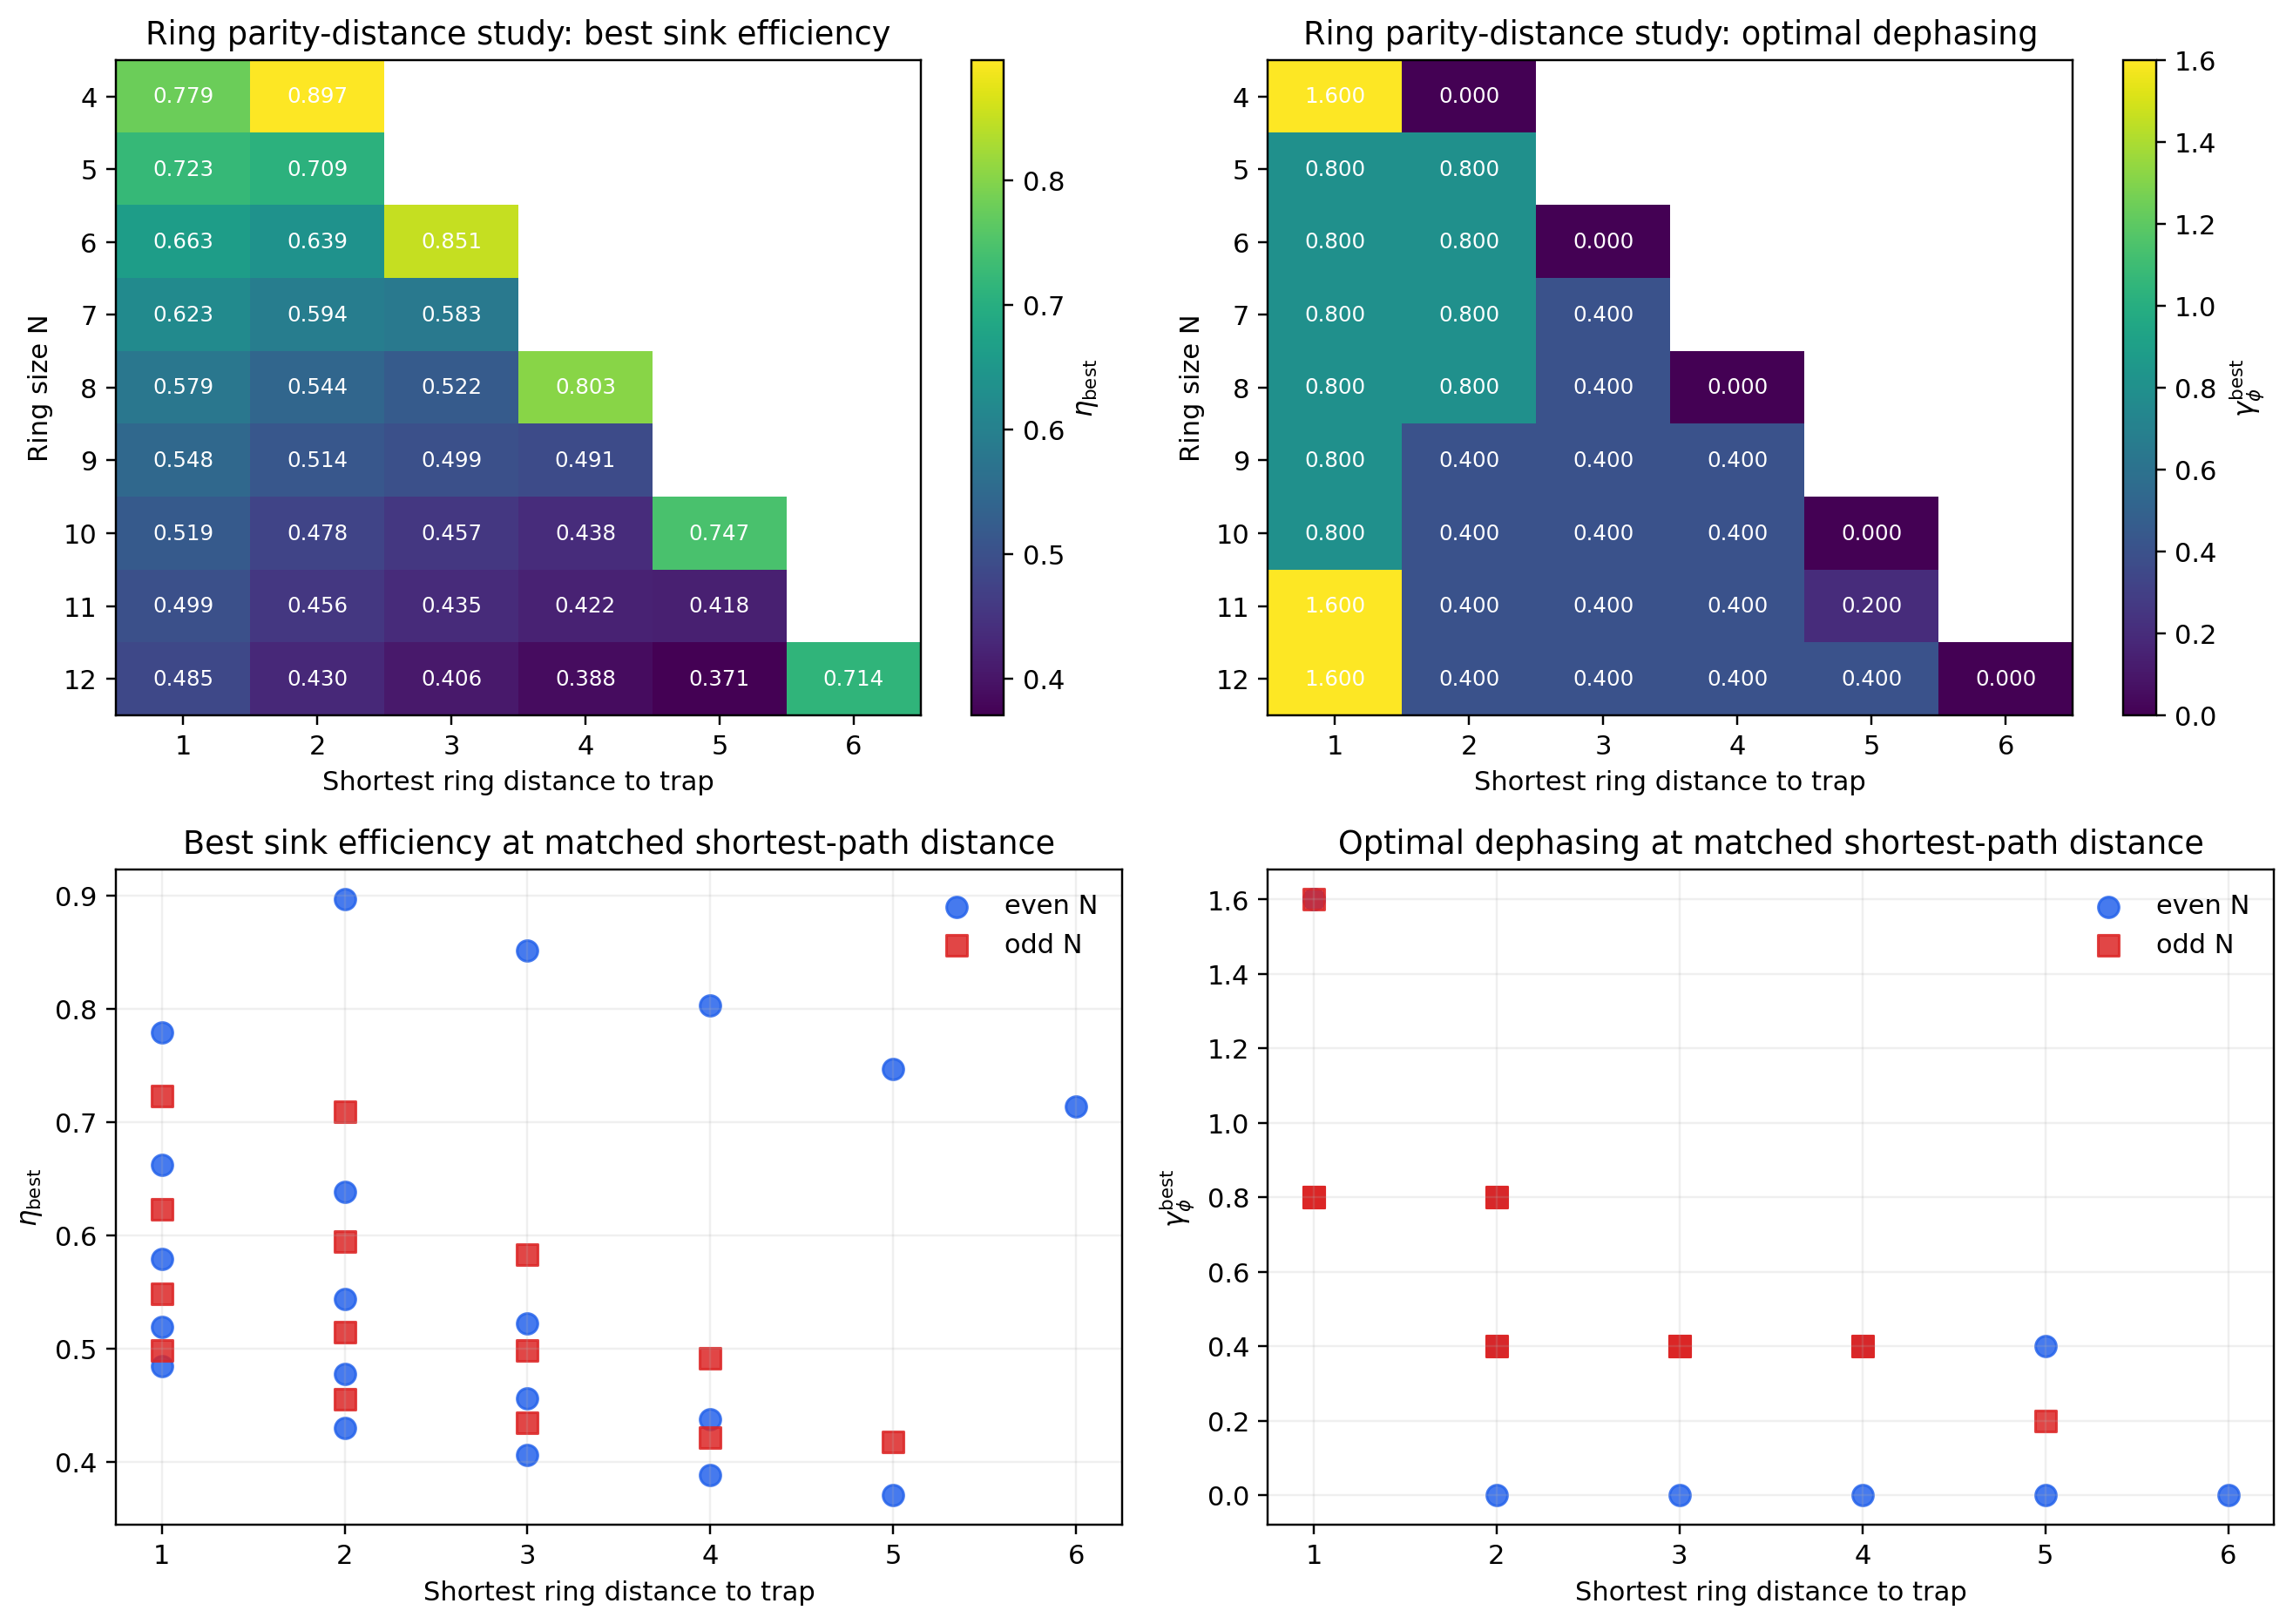
\includegraphics[width=0.86\textwidth]{../../outputs/transport_networks/targeted_studies/latest/figures/ring_parity_distance.png}
\caption{Controlled ring study that separates ring-size parity from shortest-path distance to the trap. Top panels: heat maps of best efficiency and optimal dephasing over $(N,d)$. Bottom panels: matched-distance comparisons between odd and even rings.}
\end{figure}

\begin{figure}[t]
\centering
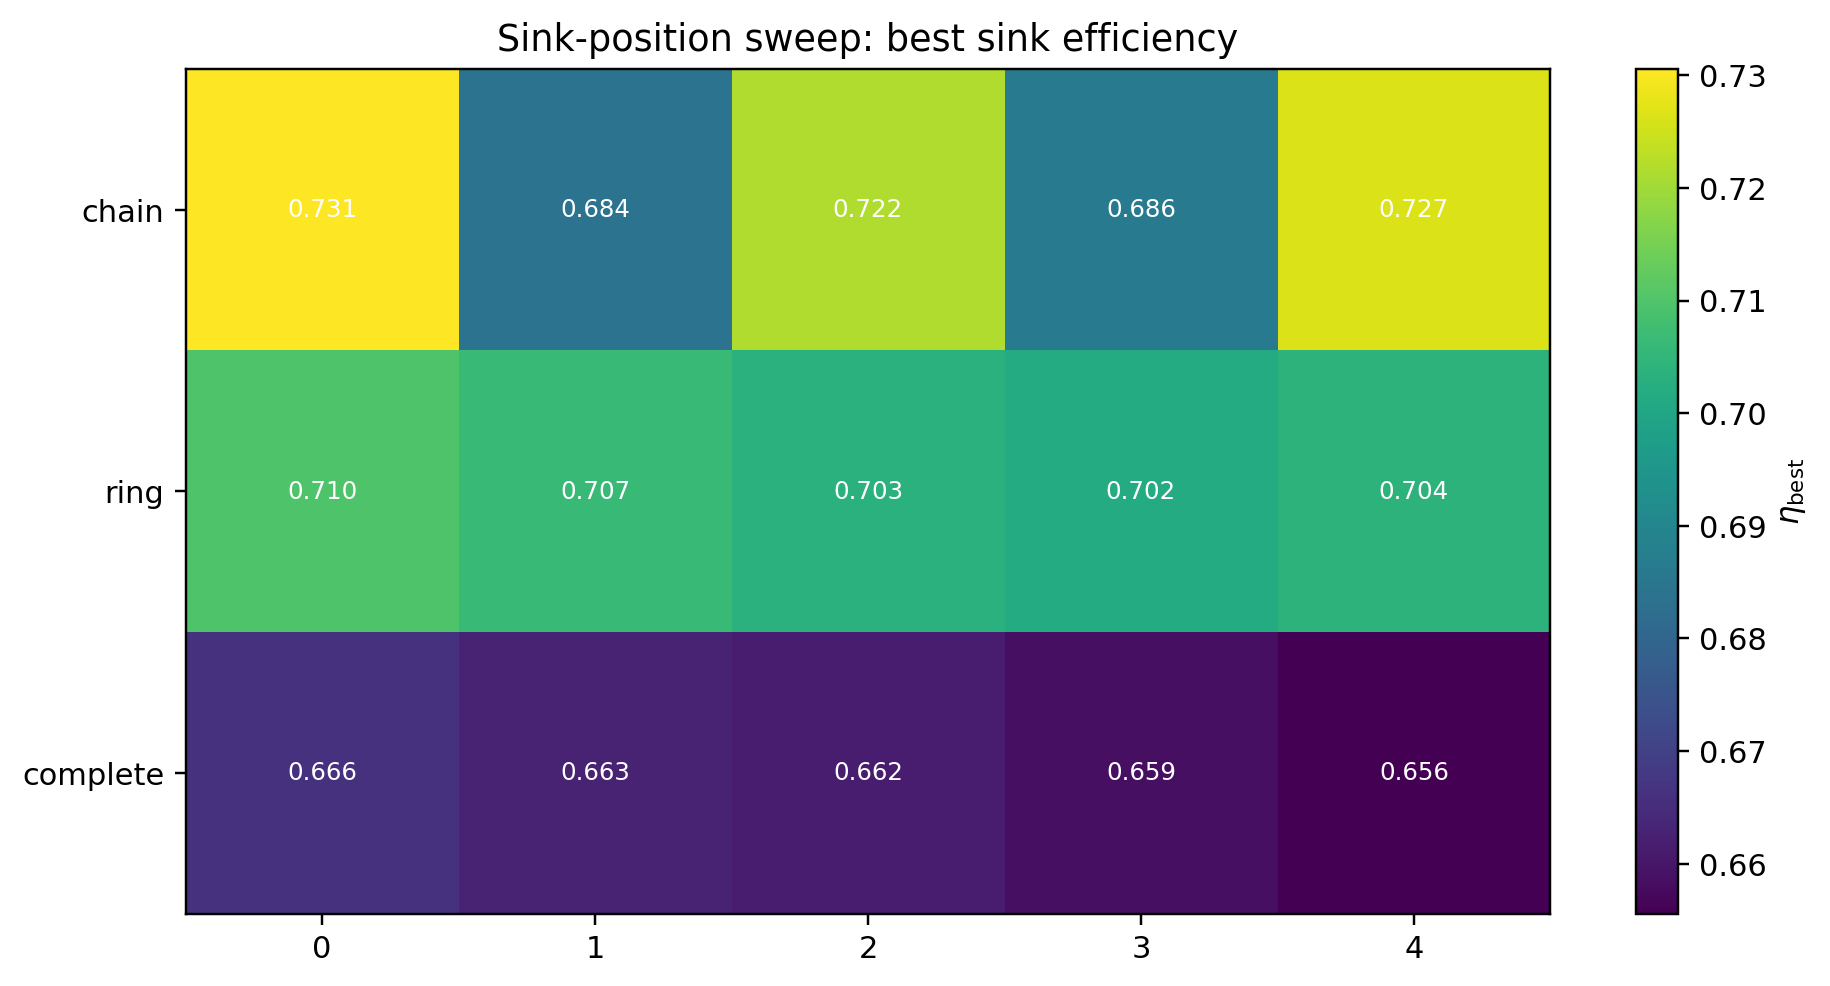
\includegraphics[width=0.48\textwidth]{../../outputs/transport_networks/targeted_studies/latest/figures/sink_position_eta_heatmap.png}
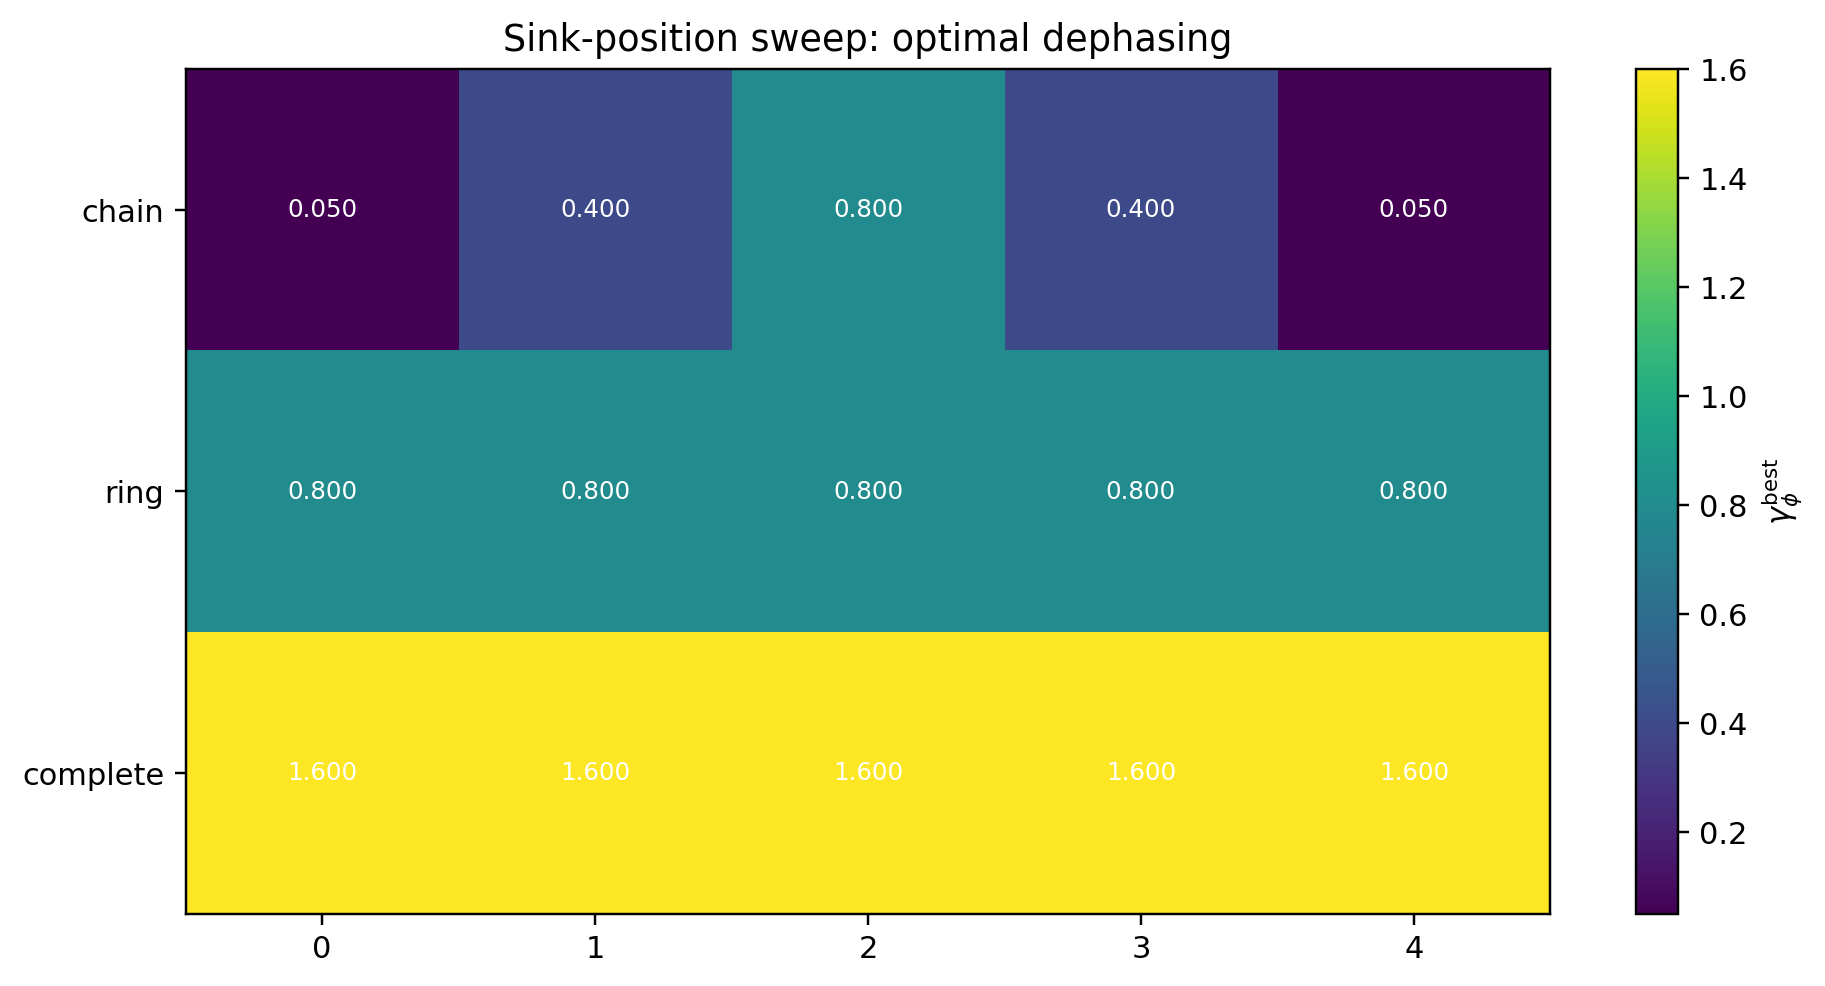
\includegraphics[width=0.48\textwidth]{../../outputs/transport_networks/targeted_studies/latest/figures/sink_position_gamma_heatmap.png}
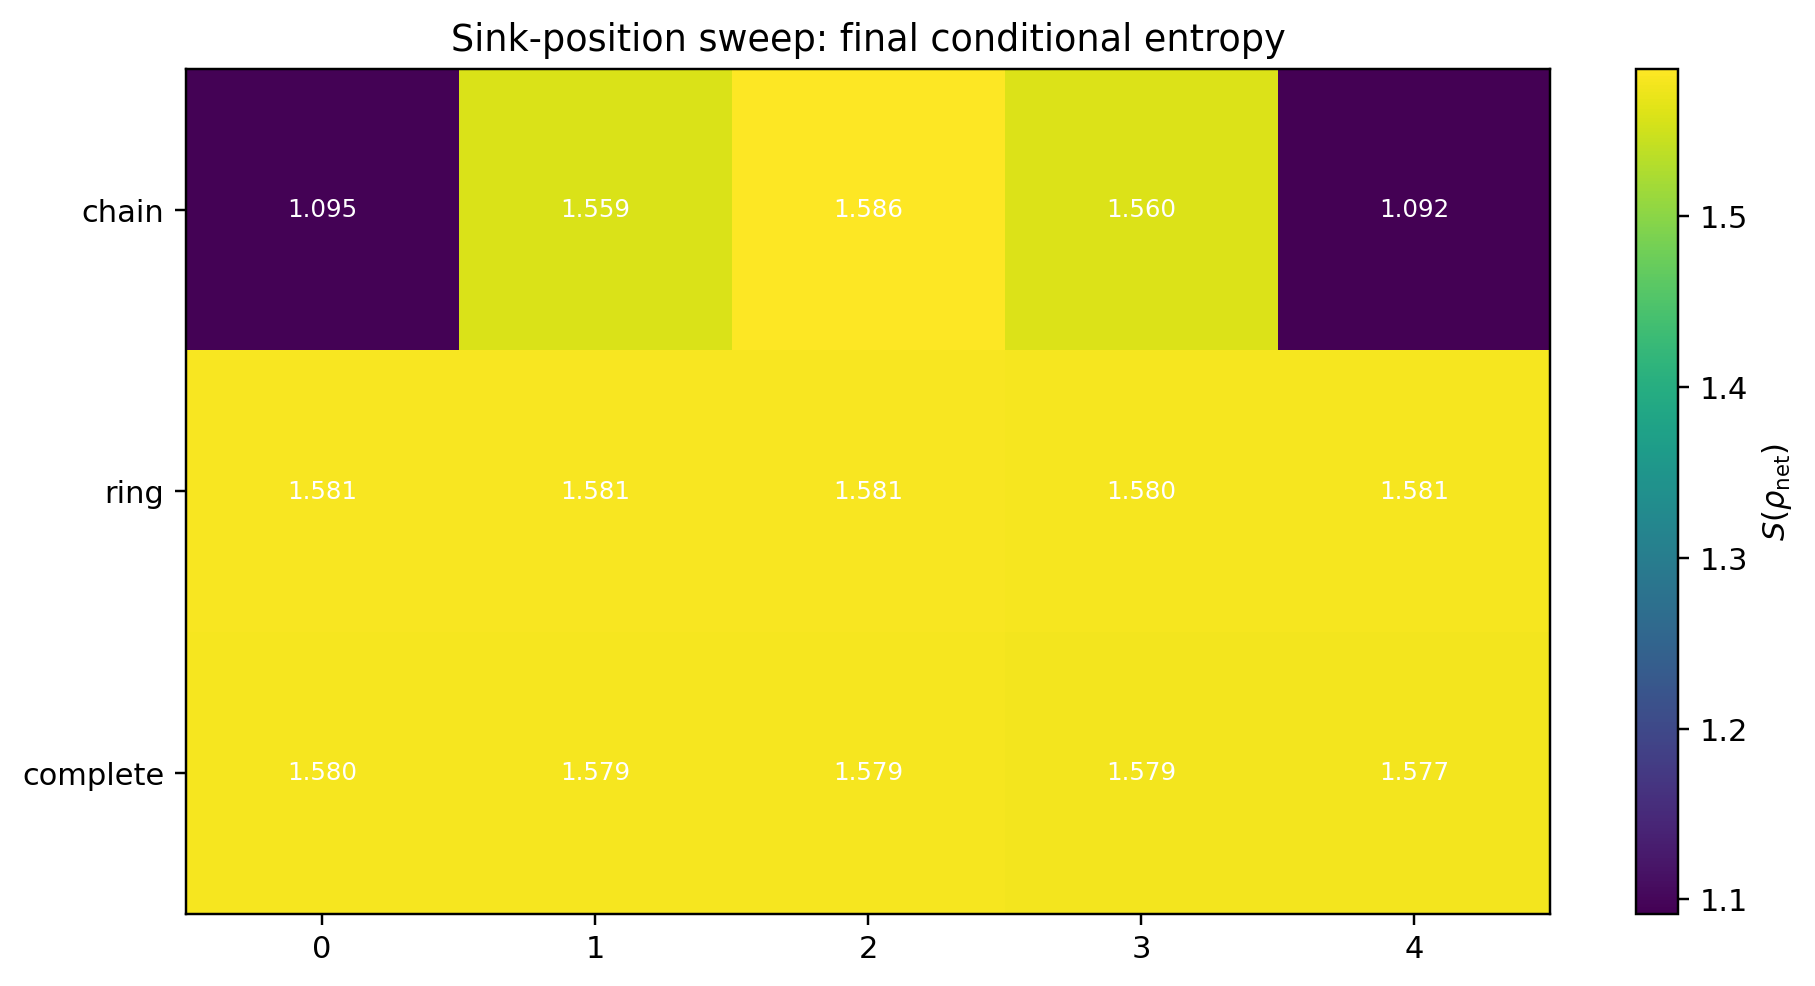
\includegraphics[width=0.48\textwidth]{../../outputs/transport_networks/targeted_studies/latest/figures/sink_position_entropy_heatmap.png}
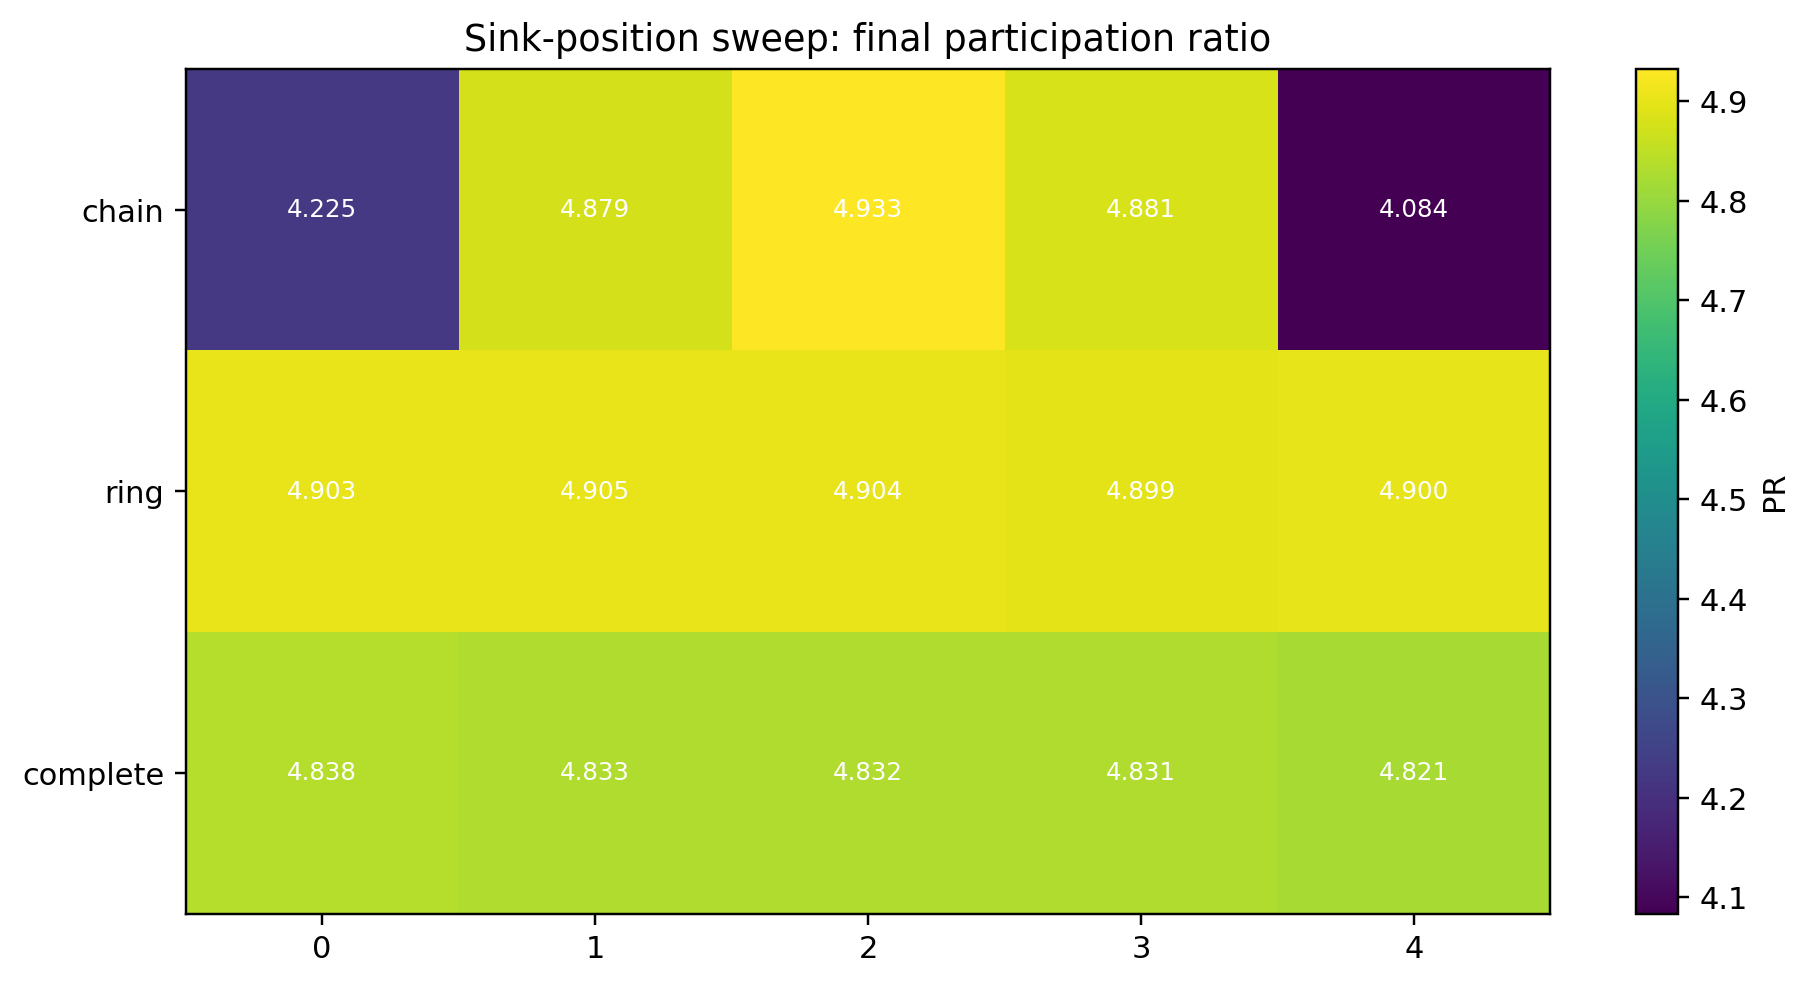
\includegraphics[width=0.48\textwidth]{../../outputs/transport_networks/targeted_studies/latest/figures/sink_position_participation_heatmap.png}
\caption{Sink-position sweep. Top-left: best transport efficiency. Top-right: optimal dephasing. Bottom-left: final conditional entropy. Bottom-right: final participation ratio. The sweep uses a 32-seed disorder ensemble.}
\end{figure}

\begin{figure}[t]
\centering
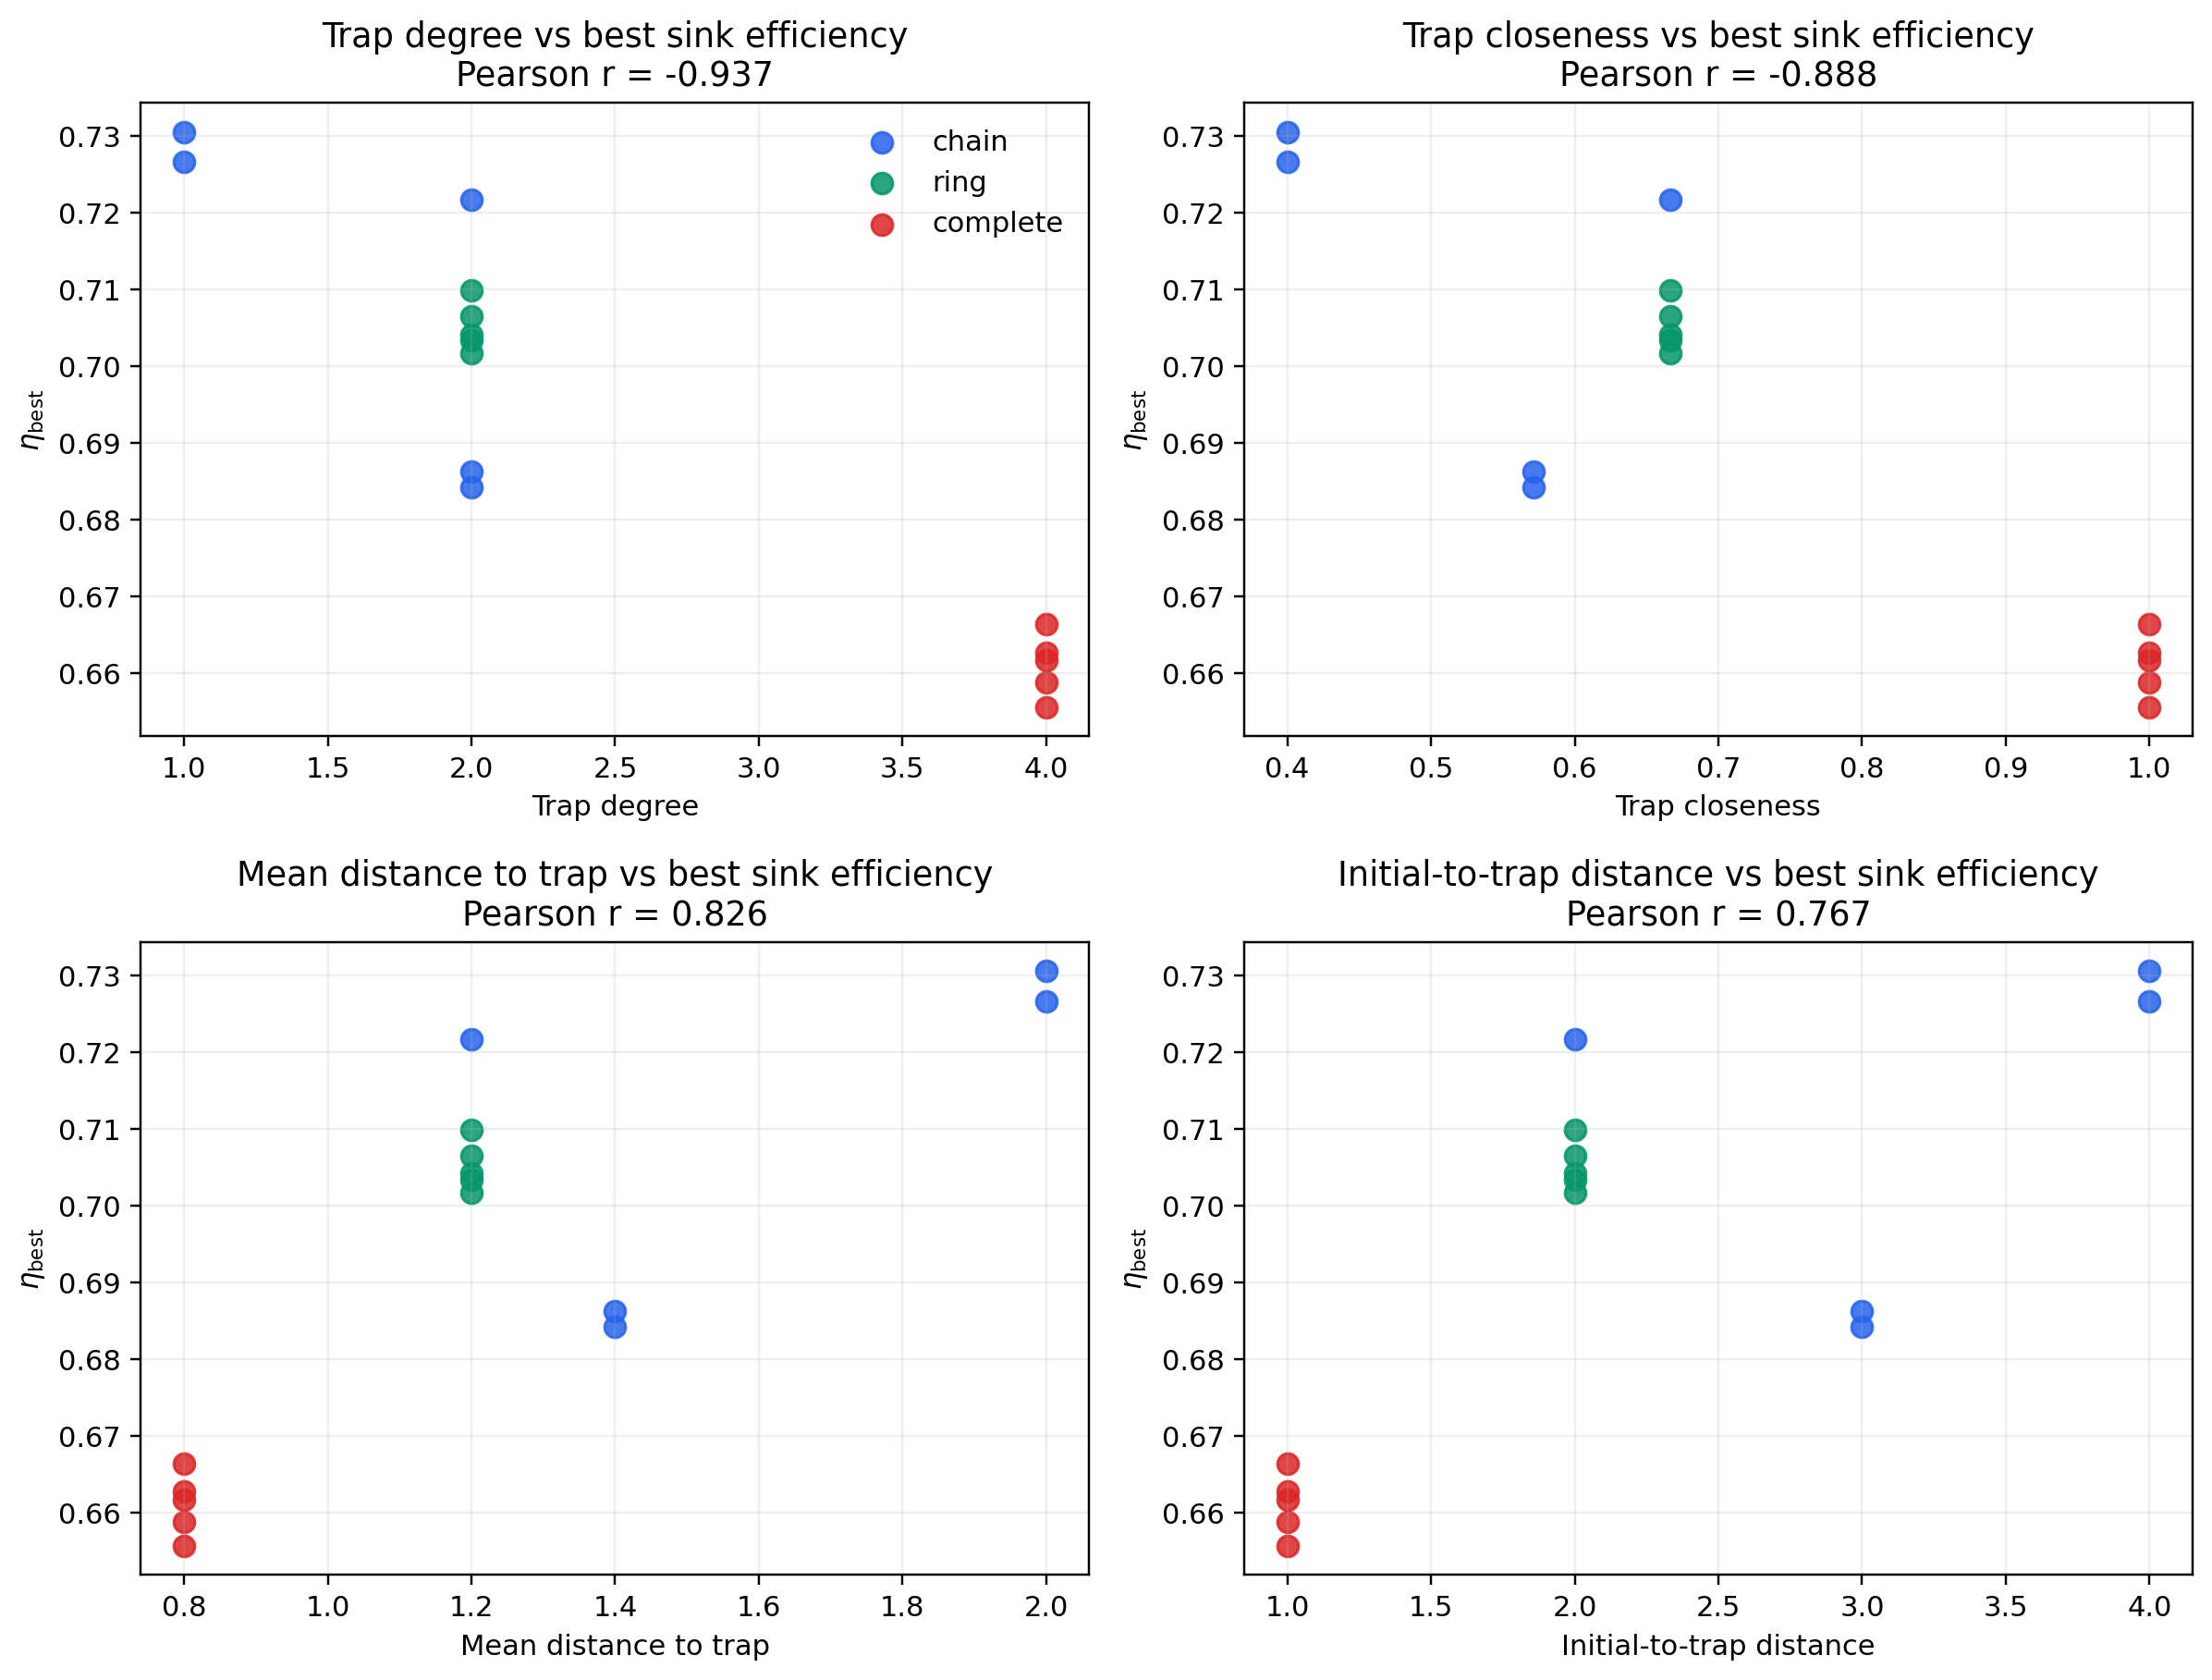
\includegraphics[width=0.86\textwidth]{../../outputs/transport_networks/targeted_studies/latest/figures/sink_position_metric_correlations.png}
\caption{Correlations between graph metrics of the trap node and the best sink efficiency in the sink-position sweep. These scatter plots are the first bridge from purely topological labels to quantitative transport predictors.}
\end{figure}

\subsection{Refined chain-disorder crossover}
The original phase-slice study suggested that the chain changed regime between $W/J=0.4$ and $W/J=0.8$. We therefore refined the disorder grid locally with a pilot ensemble of 64 seeds.
The first non-coherent optimum in the refined scan appears at $W/J=0.74$, where the best regime becomes intermediate and $\gamma_\phi^{\mathrm{best}}=0.020$.
This is the strongest current candidate for a genuine crossover line in the $(W/J,\gamma_\phi/J)$ plane. It is not yet a final claim because the targeted follow-up still needs a local refinement of the disorder axis around the transition and a convergence check of the inferred boundary against independent ensemble resampling.

\subsection{Refined ring-size sweep}
The ring was rescanned over a denser set of sizes in order to test whether the previously observed alternation with $N$ was accidental or structural.
In the current refined data, coherent-optimal rings appear at $N=[4, 6, 8, 10, 12]$ and intermediate-optimal rings appear at $N=[5, 7, 9, 11]$. That pattern is consistent with a parity/symmetry effect. The next question is whether this alternation survives after controlling explicitly for shortest-path distance to the trap.

\subsection{Ring parity versus sink distance}
To separate parity from geometry, we fixed the initial site and rescanned clean rings over unique shortest-path distances to the trap. This removes the ambiguity between ``odd versus even ring'' and ``near versus far sink''.
At distance $d=1$, the mean best efficiency is 0.605 for even rings and 0.598 for odd rings, with even-minus-odd difference +0.007. The corresponding optimal dephasing difference is +0.120.
At distance $d=2$, the mean best efficiency is 0.598 for even rings and 0.568 for odd rings, with even-minus-odd difference +0.029. The corresponding optimal dephasing difference is -0.120.
At distance $d=3$, the mean best efficiency is 0.559 for even rings and 0.505 for odd rings, with even-minus-odd difference +0.054. The corresponding optimal dephasing difference is -0.100.
At distance $d=4$, the mean best efficiency is 0.543 for even rings and 0.457 for odd rings, with even-minus-odd difference +0.086. The corresponding optimal dephasing difference is -0.133.
At distance $d=5$, the mean best efficiency is 0.559 for even rings and 0.418 for odd rings, with even-minus-odd difference +0.141. The corresponding optimal dephasing difference is +0.000.
The strongest clean ring point in this controlled study occurs at $N=4$, distance $d=2$, with $\eta_{\mathrm{best}}=0.897$ and $\gamma_\phi^{\mathrm{best}}=0.000$.
If matched-distance odd and even rings remain separated, that points to a genuine parity/size effect. If they collapse onto the same trend, then the original alternation was mostly a distance-to-target effect.

\subsection{Sink-position sweep}
The trap site was varied while keeping the topology fixed. For each trap position we again optimized over dephasing and used a 32-seed disorder ensemble.
For the chain topology, the best mean transport occurs at trap site 0, with $\eta_{\mathrm{best}}=0.731$ and $\gamma_\phi^{\mathrm{best}}=0.050$.
For the ring topology, the best mean transport occurs at trap site 0, with $\eta_{\mathrm{best}}=0.710$ and $\gamma_\phi^{\mathrm{best}}=0.800$.
For the complete topology, the best mean transport occurs at trap site 0, with $\eta_{\mathrm{best}}=0.666$ and $\gamma_\phi^{\mathrm{best}}=1.600$.
This is the first direct indication that graph topology alone is not the full story: the geometric role of the target node also matters and should be correlated next with degree, closeness, and graph distance to the initial site.
In the present sweep, the Pearson correlations with best sink efficiency are: trap degree = -0.937, trap closeness = -0.888, mean distance to trap = 0.826, and initial-to-trap distance = 0.767.

\subsection{What looks genuinely new enough to pursue}
At the present stage, the most credible candidates for publishable new results are: (i) a disorder-induced crossover line for the chain, (ii) a topology- and sink-position-dependent transport atlas in normalized variables, and (iii) a robustness ranking that reports both mean efficiency and ensemble spread.
